\section{Particle Identification and Event Selection}\label{protonid}
%The next line produces an indented paragraph to start the document
 %unit.  The LaTeX defaults start most units without indentations.
\hspace{\parindent}
Outline the analysis section.

%%%%%%%%%%%%%%%%%%%%%%%%%%%%%%%%%%%%%%%%%%%%%%%%%%%%%%%%%%%
% Particle Identification and Event Selection
%%%%%%%%%%%%%%%%%%%%%%%%%%%%%%%%%%%%%%%%%%%%%%%%%%%%%%%%%%%
\subsection{Particle Identification}
  After the particle tracks are reconstructed, we use a predictive model to
  classify proton tracks. The inputs to the model are the reconstructed
  physical variables, and the output is the probability that the track is from
  a proton vs. some other particle. There are many predictive models that we
  can use, each with advantages and disadvantages. We chose gradient-boosted
  decision trees for a few main reasons: they are easily interpretable, the
  inputs can be a mix of numeric and categorical variables, and boosted
  decision trees perform well at identifying a small signal in a large
  background.  Each tree is essentially a series of cuts based on physical
  variables which have been fine-tuned to increase the efficiency and purity of
  the final selected sample.
  \subsubsection{Reconstructed track features}
    The reconstructed features that are used as input to the classifier are
    listed below. Most of the features come directly from the track object, but
    some are created for this classifier. Each of the features used to identify
    protons either helps to separate neutrino-induced tracks from
    cosmic-induced tracks or to separate neutrino-induced proton tracks from
    other neutrino-induced particle types.

    First is a list and description of the features designed to separate
    neutrino-induced protons from other neutrino-induced particle types.
    \begin{itemize}
      \item \textbf{Number of hits:} This is the total number of hits on all
      three wire planes associated with track. When used in combination with
      track length and average energy deposited, this feature can be used to
      determine the hit and energy density of the track.
      \item \textbf{Straightness:} This is the ratio of distance between
      reconstructed end points (displacement) to reconstructed path length. It
      represents the amount of scattering a track undergoes. The value is
      always betwen zero and one with one being perfectly straight.
      \item \textbf{Cosmic score:} This is the geometry tagging cosmic score
      from Sec.~\ref{sec:tpcreco}. Tracks with a cosmic score of 1 have already
      been removed in the cosmic hit removal stage. So, this value is either 0
      (fully contained within the TPC) or 0.5 (entering or exiting the TPC).
      \item \textbf{Particle ID from energy deposited per unit length (dE/dx):}
      The PIDA and $\chi^2$ PID algorithms values described in
      Sec.~\ref{sec:tpcreco} are used.
      \item \textbf{Length:} This is the reconstructed 3D track length found by
      stepping along the trajectory points.
      \item \textbf{Start and end dQ/dx:} These are the total charge deposited
      at start and end points of track divided by the distance between hits to
      account for the angle with respect to the wires. The total charge of the
      first (or last) six track hits on each plane is summed.
      \item \textbf{End to start dQ/dx ratio and difference:} These are the
      ratio and difference of the end dQ/dx divided by (or subtracted by) the
      start dQ/dx described in the previous item.
      \item \textbf{Total dQ/dx:} This is the sum of the dQ/dx of all hits on
      all planes associated with track.
      \item \textbf{Average dQ/dx:} This is the total dQ/dx divided by the
      number of hits associated with track.
    \end{itemize}

    Next is the list and description of the features designed to separate
    neutrino-induced tracks from cosmic-induced tracks.
    \begin{itemize}
      \item \textbf{Start and end positions:} These are the reconstructed x, y,
      and z positions of start and end of the track. Tracks that start closer
      to a TPC boundary are more likely to be cosmic-induced.
      \item \textbf{$\theta$ and $\phi$:} These are the reconstructed polar and
      azimuthal angles with respect to the beam direction. Vertical tracks are
      much more likely to be cosmic-induced, while forward-going tracks are
      more likely to be from the neutrino beam.
    \end{itemize}
   
    Determining which end of a track is the beginning is difficult when a
    vertex is not observable. Since we are particularly interested in
    neutral-current elastic events with only a single proton, the direction of
    the track is a concern. A proton will deposit much more energy at the end
    of its track than at the beginning which can be used to determine the true
    direction. Since this correction is not currently implemented in pandoraNu,
    we take all reconstructed tracks that have a higher start charge than end
    charge and flip them. This means changing the saved start positions, end
    positions, $\theta$, $\phi$, start dQ/dx, end dQ/dx, and the end to start
    dQ/dx ratio and difference.
    
  \subsubsection{Boosted decision trees}\label{sec:decisiontrees}
    A decision tree can be thought of as a series of if/else statements that
    separate a data set into two or more classes as illustrated in
    Fig.~\ref{fig:dtree}. At each node of the tree, a split is chosen to
    maximize information gain until a set level of separation is reached.  At
    the terminus of the series of splits, called a leaf, a class is assigned.
    The usual parameters that can be set when creating a decision tree are: the
    maximum depth of the tree (how many layers of nodes you will allow), the
    minimum split size (how many data points do you require to keep splitting),
    and minimum leaf size (how small does a leaf have to be before you stop). 
    \begin{figure}[ht]
      \centering
      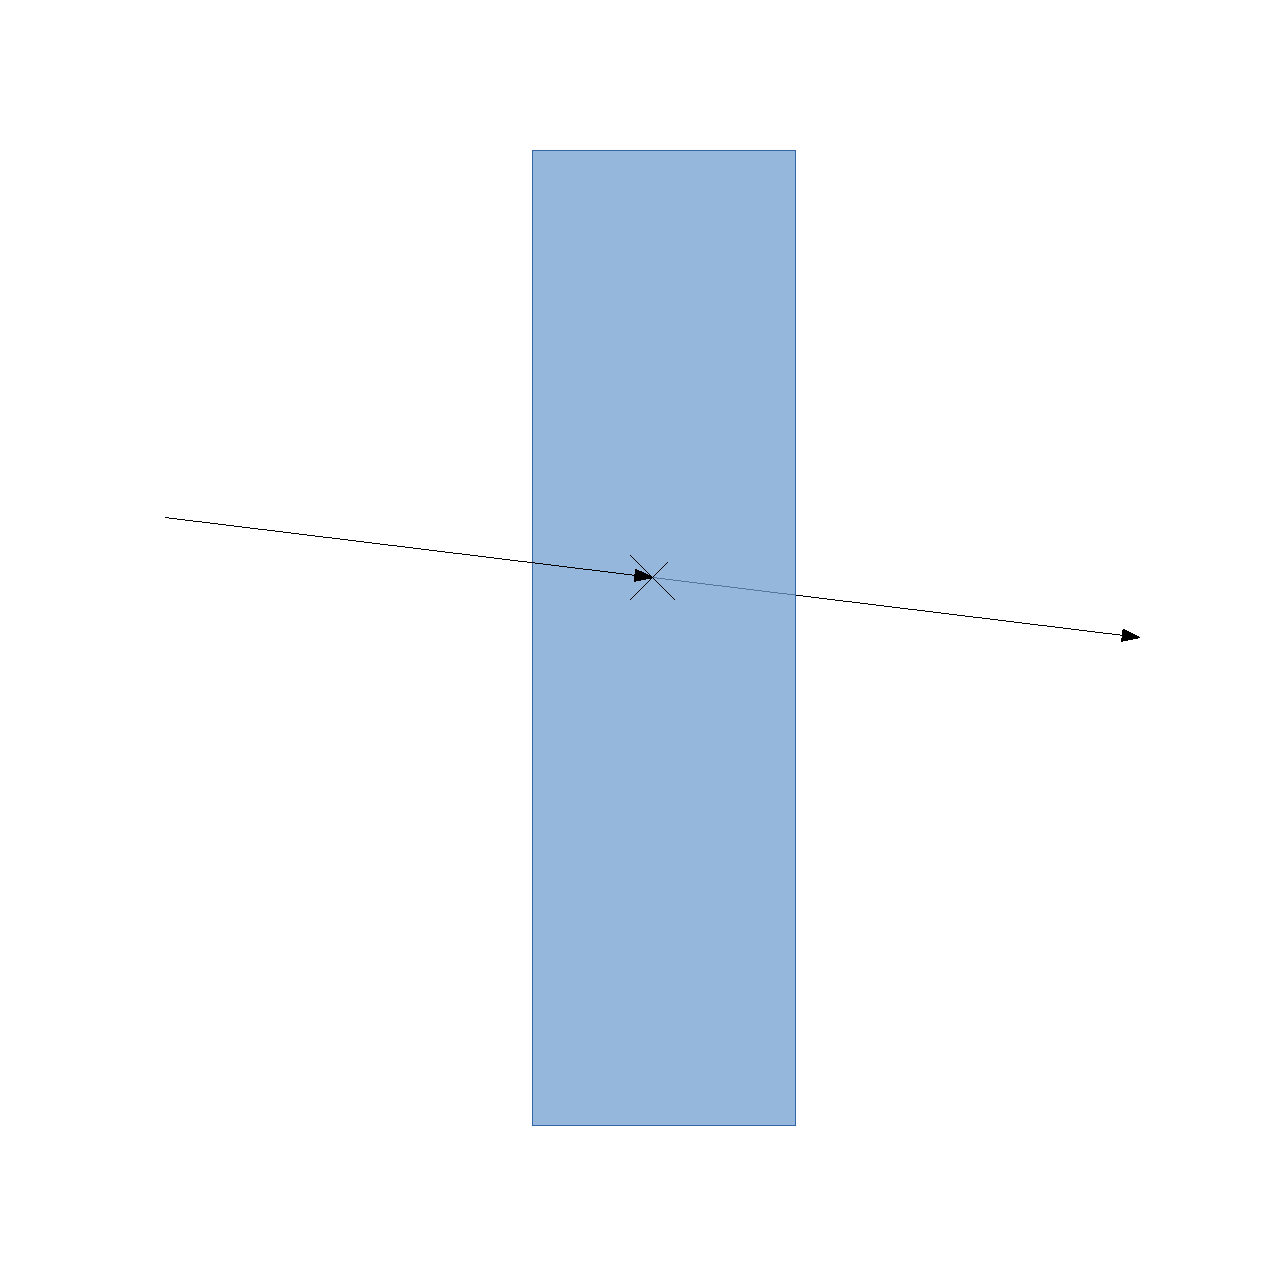
\includegraphics[angle=0,width=4in]{figures/bz.pdf}
      \caption{Graphical example of a decision tree.}
      \label{fig:dtree}
    \end{figure}
    
    A single tree can easily overfit a data set if it is at all complex, and
    its output is just a class label. Gradient-boosting addresses both of these
    issues by combining many weak classifiers into a strong one. Each weak
    classifier is built based on the error of the previous one. For a given
    training set, whenever a sample is classified incorrectly by a tree, that
    sample is given a higher importance when the next tree is being created.
    Mathematically, each tree is training on the gradient of the loss function.
    After all of the trees have been created, each tree is given a weight based
    on its ability to classify the training set, and the output of the
    gradient-boosted decision tree classifier is the probability that a sample
    is in a given class.
    
    The gradient-boosted decision tree software package we use is
    XGBoost~\cite{xgboost}. There are two types of classifiers we can use to
    separate protons from other tracks: binary and multiclass. Both classifiers
    are trained on all types of reconstructed tracks. A binary classifier
    classifies each track as either a proton or not a proton, and a multiclass
    classifier classifies a track as one of many types including a proton. We
    choose to use multiclass because the information about non-proton tracks is
    useful for event identification. The five classes that we train the
    decision trees to classify are protons (both BNB and cosmic), BNB muons,
    BNB pions, BNB electrons/photons, and all non-proton cosmics.
    
    The decision trees were trained to select protons in general. The target
    class contains all protons from BNB interactions, as well as cosmic
    protons. However, the choice of track features and most of the improvements
    that were made were done with the goal of a high efficiency for isolated
    protons and cosmic rejection.

  \subsubsection{Training}
    Describe the training sets. What samples were used, how many of everything,
    and all hyperparamter settings. Describe hyperparameter optimization. 
  \subsubsection{Performance}
    Show efficiency, accuracy, itemize backgrounds.
    Discuss reasons for different backgrounds.


%%%%%%%%%%%%%%%%%%%%%%%%%%%%%%%%%%%%%%%%%%%%%%%%%%%%%%%%%%%
% Neutral Current Elastic Proton Event Selection
%%%%%%%%%%%%%%%%%%%%%%%%%%%%%%%%%%%%%%%%%%%%%%%%%%%%%%%%%%%
\subsection{Event Selection}\label{sec:selection}
  Need to select both NCE and CCQE events.
  Use particle ID plus reconstructed flashes.
  Exactly how we select NCE events 


%%%%%%%%%%%%%%%%%%%%%%%%%%%%%%%%%%%%%%%%%%%%%%%%%%%%%%%%%%%
% Efficiency and Background Estimation
%%%%%%%%%%%%%%%%%%%%%%%%%%%%%%%%%%%%%%%%%%%%%%%%%%%%%%%%%%%
\subsection{Efficiency and Background Estimation}\label{sec:effbg}
  \subsubsection{Event selection efficiency}
    Efficiency due to TPC, PMT software trigger, reconstruction, proton ID,
    event selection, etc. This includes efficiency due to proton reinteracting
    in the nucleus and other nuclear effects.
  \subsubsection{Beam Induced Dirt Background}
    Discuss dirt neutrons, how they happen and estimated rates and energy
    distributions.  Show how well we can seperate or understand them. Show any
    sort of data-driven correction we did to dirt neutron background and how it
    affects our uncertainty. Talk about how well we can tag cryostat neutrons
    with the PMTs.
  \subsubsection{Beam Induced TPC Background}
    Talk about neutral-current elastic neutrons that are produced in the TPC
    and how their distributions differ from NCEp ones. Also include BNB
    backgounds (CCQE where muon wasn't reconstructed, NCpi0, etc.) Discuss how
    the optical signal would be different for each of these.
  \subsubsection{Cosmic Background}
    Discuss the difference between cosmic tracks and beam proton tracks. How do
    we separate them? What is the rate?


%%%%%%%%%%%%%%%%%%%%%%%%%%%%%%%%%%%%%%%%%%%%%%%%%%%%%%%%%%%
% Ratio of Cross Sections
%%%%%%%%%%%%%%%%%%%%%%%%%%%%%%%%%%%%%%%%%%%%%%%%%%%%%%%%%%%
\subsection{Ratio of NCEp to CCQEn Cross Sections}\label{sec:ratios}
  Show how the ratio gets rid of a lot of measurement uncertainty like beam
  flux and efficiencies. Give exact equation that we will be using for
  analysis. Show how $\Delta s$ is still large at low $Q^2$.
  \subsubsection{Sources of Measurement Uncertainty}
    TPC efficiency: If ionization electrons actually reach the
    TPC and leave a signal.
    PMT trigger efficiency: Refer back to PMT trigger studies. Give uncertainty
    due to on signal.
    Reconstruction efficiency: Refer back. Give uncertainty on signal.
  \subsubsection{Quantifying Uncertainty on Ratio}\label{errorcalc}
    Calculate exact uncertainty and show it here.
  \subsubsection{Model uncertainty}\label{sec:modeluncertainty}
    Nuclear effects and FSI. Discuss. Discuss which values are varied and by
    how much? Refer to reweighting section. 

